% \usepackage{algpseudocode}
% \usepackage{algorithm}

The multigrid method is a scheme applied to solving a linear equation system with iterative solvers. It provides a convergence acceleration that improves the performance of these iterative solvers using grid coarsening \citep{fedorenko1973iterative} \citep{trottenberg2000multigrid}. In practice, it can be implemented as a standalone method or as a preconditioner for other iterative methods such as the conjugate gradient method \citep{tatebe1993multigrid}. Various multigrid methods are used in different branches of applied mathematics and engineering. such as electromagnetics \citep{stolk2014multigrid} and fluid dynamics \citep{adler2016monolithic}.  

The two important components of multigrid methods are the restriction and prolongation operators which transfer information between fine grids and coarse grids. These operators are typically based on linear interpolation procedures and are connected through variational properties \citep{10.5555/357695} to ensure optimal coarse-grid correction in the $A^h$-norm with $A^h$ being the left-hand side of the linear system defined on the fine grid. The multigrid method can be also applied to the SBP-SAT method with specific grid transfer operators. In this section, we will provide a brief review of the multigrid method and its implementation. We consider the following steady-state problem:

\begin{align}
    Lu = f, &\text{ in }  \text{$\Omega$}  \label{stead-state-problem}\\
    Hu = g, &\text{ on } \partial\text{$\Omega$}
    \label{stead-state-problem2}
\end{align}

where $L$ is a differential operator on domain \text{$\Omega$},  and $H$ is a boundary operator on the boundary $\partial$\text{$\Omega$}. This is a generalization of many linear systems with various boundary conditions. 

\subsubsection{The multigrid algorithm}
In general, the construction of a multigrid consists of the following four basic steps:

\begin{enumerate}
    \item Fine-grid discretization
    \item Error smoothing
    \item Coarse-grid correction
    \item Fine-grid update
\end{enumerate}

Different combinations of these steps result in different multigrid schemes. The most simple scheme is a two-level multigrid V cycle. We will expand these four steps in the following sections.

\subsubsection{Fine-grid discretization}
Consider a \textit{fine grid} meshing \text{$\Omega$}$_1$ on \text{$\Omega$}. A discrete linear system associated to \autoref{stead-state-problem} on this fine grid \text{$\Omega$}$_1$ has the general form 

\begin{align}
    L_1 \mathbf{u} = \mathbf{F}
    \label{fine-grid-disc}
\end{align}

where $L_1$ is the discrete version of the operator $L$ in \autoref{stead-state-problem} which also include boundary conditions in \autoref{stead-state-problem2}. The vector \textbf{F} approximates $f$ on the grid points of \text{$\Omega$}$_1$ which already incorporates data for the boundary condition\textbf{g} in \autoref{stead-state-problem2}. \textbf{u} is the discretization of the solution $u$ in the steady-state problem. We assume $L_1$ to be positive definite which also implies that $L_1$ is invertible. This is property is usually satisfied from discretization methods. 

\subsubsection{Error smoothing}
Error smoothing is required prior to grid coarsening. Suppose we have an initial guess $\mathbf{u}^0$, the iterative approach towards the solution to \autoref{fine-grid-disc} is through solving

\begin{align}
    \mathbf{w}_\tau + L_1 \mathbf{w}(\tau) &= \mathbf{F},\text{ }  0 < \tau < \Delta\tau \label{pseudo-march} \\
    \mathbf{w}(0) &= \mathbf{u}^{(0)} 
\end{align}

where $\Delta_t > 0$ is the \textit{smoothing step}. The solution to this equation is 
\begin{equation}
    \mathbf{w}(\Delta\tau) = e^{-L_1\Delta\tau}\mathbf{u}^{0} + (I_1 - e^{-L_1\Delta\tau})L_1^{-1}\mathbf{F}
\end{equation}
where $I_1$ is the identity matrix on \text{$\Omega_1$}, and the following condition holds for any norm if $L_1$ is positive definite
\begin{equation}
    ||\mathbf{w}(\Delta\tau) - \mathbf{u}|| < ||\mathbf{u}^{(0)} - \mathbf{u}||
\end{equation}


Smoothing technique for the solution can be defined as follows
\begin{equation}
\begin{split}
    \mathbf{w}^k &= S\mathbf{w}^{k-1} + (I_1 - S)L_1^{-1}\mathbf{F}, k = 1, \dots \nu \\
    \mathbf{w}^0 &= \mathbf{u}^0
\end{split}
\end{equation}

where $S$ is the smoother. If $S$ is an exponential smoother $S_{\text{exp}} = e^{-L_1\Delta\tau}$, this will yield the pseudo time-marching procedure in \autoref{pseudo-march}. This iterative method would converge after $\nu$ steps to 
\begin{equation}
    \mathbf{w} = S^{\nu} \mathbf{u}^0 + (I_1 - S^{\nu})L_1^{-1}\mathbf{F}
    \label{converged_iter}
\end{equation}
The convergence criteria for this procedure is mentioned in the overview of iterative methods.

\subsubsection{Coarse-grid correction}

Next, consider the error $\mathbf{e} = L_1^{-1}\mathbf{F} - \mathbf{w}$ and the residual problem
\begin{equation}
    L_1\mathbf{e} = \mathbf{F} - L_1\mathbf{w}    
    \label{residual-fine}
\end{equation}

Instead of solving this system directly, we introduce a subset of \text{$\Omega$}$_1$ called the \textit{coarse grid} \text{$\Omega$}$_2$, and solve the associated coarse grid problem on \text{$\Omega$}$_2$
\begin{equation}
    L_2\mathbf{d} = I_r(\mathbf{F} - L_1\mathbf{w})
    \label{correction_problem}
\end{equation}

This problem is obtained from the finer grid problem \autoref{residual-fine} by using the following operators

\begin{enumerate}
    \item a restriction operator $I_r:$ \text{$\Omega$}$_1$ $\xrightarrow{}$ \text{$\Omega$}$_2$
    \item a coarse-grid operator $L_2$: \text{$\Omega$}$_2$ $\xrightarrow{}$ \text{$\Omega$}$_2$
\end{enumerate}

The coarse-grid operator can be built by using the Galerkin condition
\begin{equation}
    L_2 = I_r L_1 I_p
    \label{galerkin-condition}
\end{equation}
where $I_p: $ \text{$\Omega$}$_2$ $\xrightarrow{}$ \text{$\Omega$}$_1$ is a the prolongation operator. In some situations, $L_2$ can be built independently through the direct use of discretization methods, but $I_r$ and $I_p$ needs to be carefully defined so the Galerkin condition \autoref{galerkin-condition} still holds.

The prolongation operator $I_p$ is commonly chosen through linear interpolation. Assume \text{$\Omega$}$_1$ had a grid spacing of $\Delta x = 1/N$, and \text{$\Omega$}$_2$ consists of the even grid points of \text{$\Omega$}$_1$. This leads to 

\begin{equation}
    (I_p \mathbf{v})_m= 
\begin{cases}
    v_j,& m = 2j, j = 0,\dots,N/2 \\
    \frac{1}{2} (v_j + v_{j+1}),              & m = 2j + 1, j = 0,\dots,N/2
\end{cases}
\end{equation}

As we already define the prolongation operator, the restriction operator is given as 
\begin{equation}
    I_r = I_p^T / C
\end{equation}
which is called the variational property. The C is a constant determined by the discretization method. In this problem, the value for C is 2.

\subsubsection{Fine-grid update}
Finally, we update the fine grid solution with correction \textbf{d} as
\begin{equation}
    \mathbf{u}^{(1)} = \mathbf{w} + I_p\mathbf{d}
    \label{correction-scheme}
\end{equation}
The relation \autoref{correction-scheme}, together with \autoref{converged_iter} and \autoref{correction_problem} provides an iterative method for solving the steady-state problem 
\begin{align}
    \mathbf{u}^{n+1} = M\mathbf{u}^{n} + N\mathbf{F}
\end{align}
where 
\begin{align}
    M &= CS^\nu \\
    C &= I_1 - I_pL_2^{-1}I_rL_1 \\
    N &= (I_1 - M)L_1^{-1}
\end{align}
M is called the multigrid iteration matrix here and C is referred to as the coarse grid correction operator. Here, M plays a central role in the convergence of the iterative method. We can see this by the definition of the error at step n $\mathbf{e}^{(n)} = \mathbf{u}^{(n)} - L_1^{-1}\mathbf{F}$ as we get
\begin{align}
    \mathbf{e}^{(n+1)} = M\mathbf{e}^{(n)}
\end{align}
which again leads to the same convergence criteria for the iterative method depending on the spectral radius of $M$.

To demonstrate the actual process of a multigrid scheme, we use the following two-grid correction scheme as an example

\begin{enumerate}
    \item Relax $\nu_1$ times on $L_1^h\mathbf{u}^{(1)} = \mathbf{F}^{(1)}$ on \text{$\Omega$}$_1$ with the initial guess $\mathbf{v}^{1}$
    \item Compute the fine-grid residual $\mathbf{r}^{(1)} = \mathbf{F}^(1) - L_1\mathbf{v}^{(1)}$ and restrict it to the coarse grid by $\mathbf{r}^{(2)} = I_r \mathbf{r}^{(1)}$
    \item Solve $L_2\mathbf{e}^{(2)} = \mathbf{r}^{(2)}$ (or relax $\nu_1$ times) on \text{$\Omega$}$_2$
    \item Interpolate the coarse-grid error to the fine grid by $\mathbf{e}^{(1)} = I_p\mathbf{e}^{(2)}$ and correct the fine-grid approximation by $\mathbf{v}^{1} \xleftarrow{} \mathbf{v}^{(1)} + \mathbf{e}^{(1)}$
    \item Relax $\nu_2$ times on $L_1\mathbf{u}^{(1)} = \mathbf{F}^{(1)}$ on \text{$\Omega$}$_1$ with the initial guess $\mathbf{v}^{(1)}$
\end{enumerate}

There are more schemes for multigrid, and the main schemes are summarized in\autoref{fig:multigrid_scheme}.
\begin{figure}
    \centering
    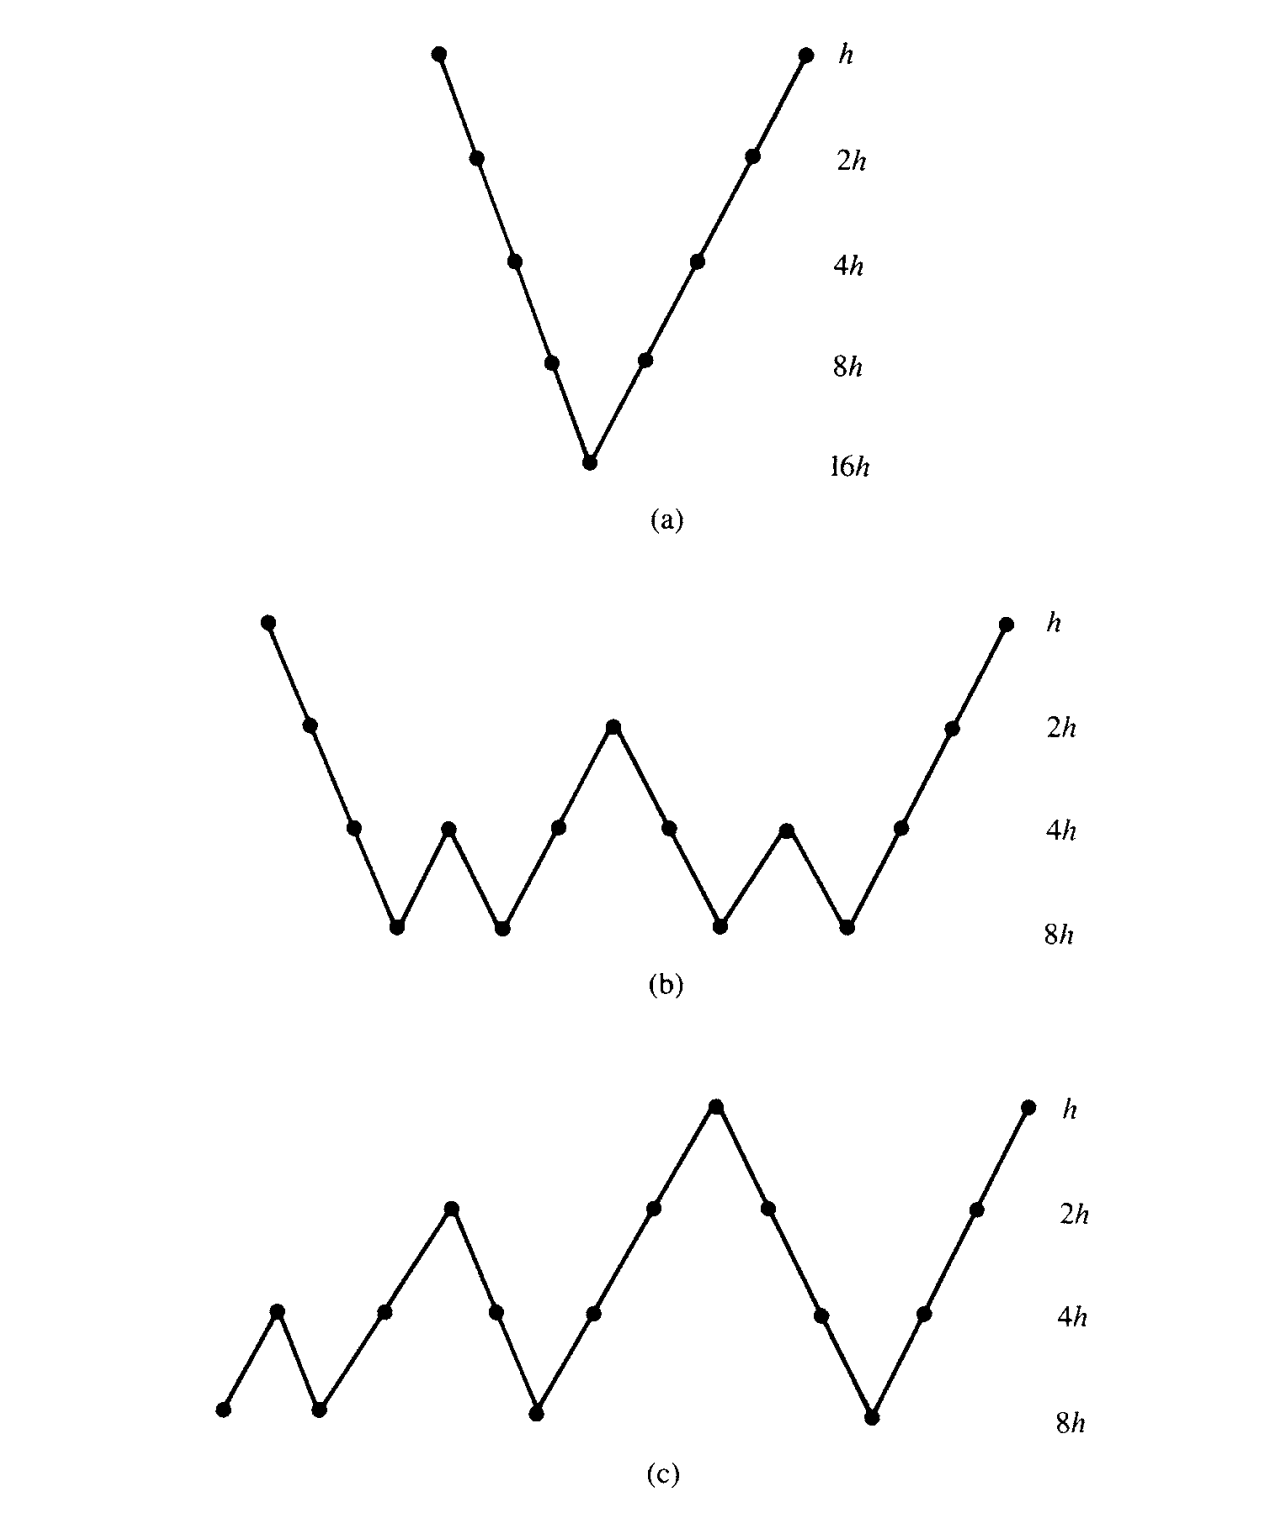
\includegraphics[width=\linewidth]{figures/multigrid_scheme.png}
    \caption{Schedule of grids for (a) V-cycle, (b) W-cycle, and (c) FMG scheme,
all on four levels. \citep{10.5555/357695}}
    \label{fig:multigrid_scheme}
\end{figure}

Earlier work in multigrid relies on the geometric structure to construct coarse problems, thus this approach is called geometric multigrid.  In problems where the computational domain is not composed of well-structured meshes, the multigrid method can be also applied via algebraic operators rather than a geometric grid.  This approach is called the algebraic multigrid. We will cover this approach in the next subsection.

\subsection{Algebraic Multigrid}
  The classical multigrid formed around the geometric structure has been generalized that the multigrid is analyzed in terms of the matrix properties \citep{mccormick1982multigrid}. This algebraic approach to theory was further extended to form the basis for much of the early development that led to the so-called Ruge-St{\"u}ben or classical algebraic multigrid (CAMG) method \citep{brandt1986algebraic,mandel1988algebraic,ruge1987algebraic}. A detailed overview of the algebraic multigrid can be found in this recent paper \citep{xu2017algebraic}. Here, we want to present it more concisely.
  We begin this subsection with the following theorem in linear algebra taken from \citep{10.5555/357695}.
\begin{theorem}[Solvability and the Fundamental Theorem of Linear
Algebra]
Suppose we have a matrix $A \in \mathbf{R}^{m\times n}$. The fundamental theorem of linear algebra states that the range (column space) of the matrix, $\mathcal{R}(A)$, is equal to the orthogonal
complement of $\mathcal{N}(A^T)$, the null space of ${A}^{T}$. Thus, spaces $\mathbf{R}^m$ and $\mathbf{R}^n$ can be
orthogonally decomposed as follows:
\begin{align}
    \mathbf{R}^m &= \mathcal{R}(A) \oplus \mathcal{N}(A^T)\\
     \mathbf{R}^n &= \mathcal{R}(A) \oplus \mathcal{N}(A)
\end{align}
For the equation $A\mathbf{u}=\mathbf{f}$ to have a solution, it is necessary that the vector $\mathbf{f}$ lie in $\mathcal{R}(A)$. Thus, an equivalent condition is that $\mathbf{f}$ be orthogonal to every vector in $\mathcal{N}(A^T)$. For the equation $A\mathbf{u}=\mathbf{f}$ to have a \textit{unique} solution, it is necessary that $\mathcal{N}(A) = \{\mathbf{0}\}$. 
Otherwise, if $\mathbf{u}$ is a solution and $\mathbf{v} \in \mathcal(A)$, then $A(\mathbf{u} + \mathbf{v}) = A\mathbf{u} + A\mathbf{v} = \mathbf{f} + \mathbf{0} = \mathbf{f}$, so the solution is not unique.
\end{theorem}
This is another point to view the coarse-grid correction scheme, and this leads to the algebraic multigrid. More theories related to this topic and the spectral picture of multigrid can be found in \citep{10.5555/357695}.

The unique aspect of the CAMG is that the coarse problem is defined on a subset of the degrees of freedom of the initial problem, thus resulting in both coarse and fine points, which leads to the term CF-based AMG. A different approach to constructing algebraic multigrid is called \textit{smoothed aggregation} (SA) AMG, where collections of degrees-of-freedom define a coarse degree-of-freedom \citep{vanvek1996algebraic}. Together, CF and SA form the basis of AMG and led to several developments that extend AMG to a wider class of problems and architectures.

AMG does not depend on the geometry of the problem and discretization schemes, and due to this generalizability, it has been implemented in different forms in many software libraries. The original CAMG algorithm and its variants are available as \texttt{amg1r5} and \texttt{amg1r6} \citep{ruge1987algebraic}. A parallel implementation of the CF-based AMG can be found in the BoomerAMG package in the Hypre library \citep{yang2002boomeramg}. The Trilinos package includes \texttt{ML} as a parallel SA-based AMG solver \citep{gee2006ml}.
PETSc adopts a geometric algebraic multigrid (GAMG) based on smoothed aggregation \citep{petsc-web-page}.
Finally, PyAMG includes a number of AMG variants for testings, and Cusp distributes with a standard SA implementation for use on a GPU \citep{dalton2014cusp,bell2022pyamg}. 

\subsection{The Multigrid Method Within the SBP-SAT Scheme}
Since the SBP-SAT scheme is a framework for discretization to form a linear system, it is compatible with the multigrid method and can be accelerated using this technique. The key challenge from simply applying the common prolongation and restriction operators with the Galerkin condition \autoref{galerkin-condition} is that the summation-by-parts property would not be preserved for the coarse grid operators. In order to accurately represent the coarse-grid correction problem for the SBP-SAT scheme, a more suitable class of interpolation operators needs to be proposed. Many works have been done to address this issue \citep{ruggiu2018new,RUGGIU2018216}.

To overcome this issue, consider defining the restriction operator as 
\begin{equation}
    I_r = H_2^{-1}I_p^TH_1
    \label{eqn:interpolation_sbp}
\end{equation}
which was first introduced in \citep{RUGGIU2018216}. This involves the coarse grid SBP norm $H_2$ and is obtained by enforcing that two scalar products
\begin{align}
    (\phi_1,\psi_1)_{H_1} &= (\phi_1H_1\psi_1) \\
     (\phi_2,\psi_2)_{H_2} &= (\phi_2H_2\psi_2)
\end{align}
are equal for $\phi_1 = I_p\phi_2$ and $\psi_2 = I_r \psi_1$. $\phi$ and $\psi$ correspond to the $\boldsymbol{u}$ and $\boldsymbol{v}$ in the previous section on iterative solvers. We use these new notations to avoid confusion with the $\mathbf{u}$ used in the previous subsection on the multigrid method. As a result, the interpolation operators $I_r$ and $I_p$ are adjoints to each other with respect to the SBP-based scalar products defined in \citep{hackbusch2013multi}.
\begin{align}
    (I_p,\xi_2,\xi_1)_{H_1} = (\xi_2,I_r\xi_1)_{H_2}
    \label{eqn:adjoint}
\end{align}

by using \autoref{eqn:interpolation_sbp}, it is possible to build pairs of consistent and accurate prolongation and restriction operators. The following definition of the SBP-preserving interpolation operators was given in \citep{RUGGIU2018216}, where the operators were used to couple SBP-SAT formulations on grids with different mesh sizes with numerical stability.



\begin{definition}
  Let the row-vectors $\mathbf{x}_1^k$ and $\mathbf{x}_2^k$ be the projections of the monomial $x^k$ onto equidistant 1-D grids corresponding to a fine and coarse grid, respectively. $I_r$ and $I_p$ are then called 2$q$-th order accurate SBP-preserving interpolation operators if $I_r\mathbf{x}_1^k - \mathbf{x}_2^k$ and $I_p\mathbf{x}_2^k - \mathbf{x}_1^k$ vanish for $k = 0, ...,2q-1$ in the interior and for $k=0,...,q-1$ at the boundaries.
\end{definition}


The sum of the orders of the prolongation and restriction operators should be at least equal to the order of the differential equation. As a consequence, the use of high-order interpolation is not required here to solve the linear system with the multigrid method. However, high-order grid transfer operators can be used in combination with high-order discretization \citep{sundar2015comparison}. 

SBP-preserving interpolation operators with minimal bandwidth are given in Appendix A. The restriction operator $I_r$, which differs from the conventional one at boundary nodes, is shown in \autoref{fig:sbp_restriction}.


\begin{figure}
    \centering
    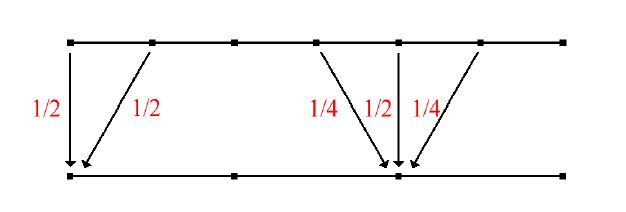
\includegraphics{figures/sbp_restriction.png}
    \centering
    \caption{The 2nd-order SBP-preserving restriction operator $I_r$}
    \label{fig:sbp_restriction}
\end{figure}




\subsubsection{SBP-preserving interpolation applied to the first derivative}
Using Galerkin condition \autoref{galerkin-condition} and SBP-preserving operators, we can construct the linear system with the multigrid method. We first consider the first derivative fine-grid SBP operator $D_{1,1}$ and its coarse-grid counterpart $D_{1,2}$ constructed as follow
\begin{equation}
    D_{1,2} = I_r D_{1,1} I_p
\end{equation}
We now show that $D_{1,2}$ preserves SBP property in such ways. To start with, we rewrite the left-hand side of the following SBP property

\begin{equation}
    (\phi,D_1\psi)_H = \phi_N\psi_N - \phi_0\psi_0 - (D_1\phi,\psi)_H
\end{equation}
with the adjoint relation \autoref{eqn:adjoint} as follows
% \begin{align}
%     (\phi_2,D_{1,2}\psi_2)_{H_2} &= (\phi_2,I_r(D_{1,1}I_p\phi_2))_{H_2} \nonumber\\&= (I_p\phi_2,D_{1,1}(I_p\psi_2))_{H_1}
% \end{align}

\begin{equation}
    (\phi_2,D_{1,2}\psi_2)_{H_2} = (\phi_2,I_r(D_{1,1}I_p\phi_2))_{H_2} = (I_p\phi_2,D_{1,1}(I_p\psi_2))_{H_1}
\end{equation}

Next, the SBP property for the finite-grid operator $D_1$ leads to
\begin{equation}
     (\phi_2,D_{1,2}\psi_2)_{H_2} = (I_p,\phi_2)_N(I_p,\psi_2)_N - (I_p,\phi_2)_0(I_p,\psi_2)_0 - (D_{1,1}(I_p\phi_2),I_p\psi_2)_{H_1}
     \label{eqn:sbp_multigrid}
\end{equation}

Both grids are conforming to the domain boundaries, and the prolongation onto the boundary nodes of the fine grid is exact. Furthermore, by applying \autoref{eqn:adjoint} to the right-hand side of \autoref{eqn:sbp_multigrid}, we obtain 
\begin{equation}
    (\phi_2,D_{1,2}\psi_2)_{H_2} = \phi_{2,N/2}\psi_{2,N/2} - \phi_{2,0}\psi_{2,0} - (D_{1,2}\phi_{2},\psi_{2})_{H_2}
\end{equation}
And we've shown that the coarse grid operator $D_{1,2}$ constructed in a such way preserves the SBP property. Also, the coarse grid first derivative SBP operator $D_{1,2}$ retains the order of accuracy of the original scheme at the interior nodes if 2$q$th order SBP-preserving interpolations are used. The proof can be found in \citep{ruggiu2018new}.

\subsubsection{SBP-preserving interpolation applied to the second derivative}
The SBP-preserving interpolation can also be applied to the second derivative operator. Similar to the proof for the first derivative operator, we can prove that the coarse grid operator constructed in such ways preserves the SBP property.

The interpolation operators in \autoref{eqn:interpolation_sbp} lead to a coarse-grid second derivative operator $D_{2,2}$ which preserves the summation-by-parts property in \autoref{eqn:2d_sbp}. We can show that by rewriting the left hand side of the \autoref{eqn:2d_sbp} for $D_{2,2}$ and the two coarse-grid functions $\phi_2$ and $\psi_2$ by using \autoref{eqn:adjoint}.
\begin{equation}
    (\phi_2,D_{2,2}\psi_2)_{H_2} = (\phi_2,I_r,D_{2,1}I_p\psi_2)_{H_2} = (I_p\phi_2,D_{2,1}I_p\psi_2)_{H_1}
\end{equation}
By applying the SBP property \autoref{eqn:2d_sbp} for the fine-grid second derivative $D_{2,1}$, we have
\begin{equation}
    (\phi_2,D_{2,2}\psi_2)_{H_2} = (I_p\phi_2)_N(SI_p\psi_2)_N - (I_p\phi_2)_0(SI_p\psi_2)_0 - (SI_p\phi_2)^TA(SI_p\psi_2)_{H_2}
\end{equation}

Both grids are conforming to domain boundaries, implying that $(I_p\phi_2)_i = \phi_{2,i/2}$ and $(SI_p\psi_2) = (S\phi_2)_{i/2}$ for $i\in\{0,N\}$. Thus 
\begin{equation}
     (\phi_2,D_{2,2}\psi_2)_{H_2} = \phi_{2,N/2}(S\phi_2)_{N/2} - \phi_{2,0}(S\phi_2)_0 - (SI_p\phi_2)^TA(SI_p\psi_2)_{H_2}
\end{equation}
where $S$ is equivalent to $\boldsymbol{d}_0^T$ which approximates the first derivative at the boundaries as discussed in the previous section on the SBP-SAT methods.

Additional proofs or propositions to SBP-preserving interpolations can also be found in  \citep{ruggiu2018new}. Furthermore, several model problems have been tested with multigrid iteration schemes using these SBP-preserving interpolations. These problems include a Poisson equation, the anisotropic elliptic problem, and the advection-diffusion problem. Numerical experiments show that the SBP-preserving interpolation improves convergence properties of the multigrid scheme for SBP-SAT discretizations regardless of the order of the discretization and smoother chosen. Moreover, the excellent performance in combination with the smoother SOR, clearly indicates that multigrid algorithms with SBP-preserving interpolation can be designed to get fast convergence. The paper mainly covers the steady model problem to compare the effect of different grid transfer operators. For time-dependent problems, the effectiveness of multigrid algorithms with these SBP-preserving interpolations needs to be tested \citep{ruggiu2018new}.


\subsection{Multigrid Preconditioned Conjugate Gradient}
In the previous sections, we introduce the classical iterative solvers and Krylov subspace methods as a solver. Moreover, we show that the classical iterative solvers can be used in the multigrid method as smoothers. And we provide the basic knowledge on preconditioners for iterative methods. However, using multigrid as a preconditioner for the conjugate gradient is an alternative approach motivated by engineering problems.

The multigrid method is a very effective iterative method for the mechanical analysis of heterogeneous material samples in \citep{hafner2006mesoscale}. However, the increase in the ratio of Young's moduli between matrix material and inclusion leads to a significantly worse condition number of the system, which slows the solution process. This could be also the result of the worse material representation on coarse grids. For a similar problem, Poisson's equation with large coefficient jumps or differences of grid spacing in coordinate transformation, the worse condition number will also lead to the slow solving process with the iterative methods mentioned above. As Poisson's equation is the key challenge in earthquake cycle simulation, an effective approach to solving linear systems with worse condition numbers is worth exploring. It has been shown that the multigrid preconditioned conjugate gradient method has a superior convergence rate over the multigrid method as a solver \citep{tatebe1993multigrid}. This approach is less dependent on the considered problem.


 The conditions of the multigrid preconditioners are examined in \citep{tatebe1993multigrid}. According to \citep{wesseling2004introduction}, the multigrid method will potentially provide a valid preconditioner if the smoother is symmetric. For a derivation of the preconditioned conjugate gradient method, we would introduce a matrix $\boldsymbol{L}$ which satisfies $\boldsymbol{M}^{-1} = \boldsymbol{L}^T\boldsymbol{L}$ as shown in \citep{wesseling2004introduction} (Our notation $\boldsymbol{M}$ is equivalent to $\boldsymbol{H}$ in the paper). The \autoref{eqn:preconditioned-system}  improves the convergence if the condition number of the preconditioned matrix $\boldsymbol{M}^{-1}\boldsymbol{A}$ is lower than that of the original matrix $\boldsymbol{A}$, which can be determined from the analysis of eigenvalues as presented in \citep{hackbusch2013iterative}. If the preconditioning matrix is exactly $\boldsymbol{M}^{-1} = \boldsymbol{A}^{-1}$, the after one iteration step, the exact solution $\boldsymbol{u}$ is found. An ideal preconditioning matrix $\boldsymbol{M}^{-1}$ should be a reasonably close approximation of $\boldsymbol{A}^{-1}$. With respect to the initial search direction, the vector $\boldsymbol{p}^0 = \boldsymbol{M}^{-1}\boldsymbol{r}^0$ would correspond to the error $-\boldsymbol{e}^0$, if $\boldsymbol{M}^{-1} = \boldsymbol{A}^{-1}$. An adequate matrix $\boldsymbol{M}^{-1}$ leads to an improved initial search direction $\boldsymbol{p}^0$. Therefore, the preconditioned conjugate gradient method applies the following start conditions
\begin{equation}
    \boldsymbol{r}^0 = \boldsymbol{f} - \boldsymbol{A}\boldsymbol{u}^0; \quad \tilde{\boldsymbol{r}}^0 = \boldsymbol{p}^0 = \boldsymbol{A}^{-1}\boldsymbol{r}^0
\end{equation}
The following equations give a preconditioned conjugate gradient method adapted from \citep{tatebe1993multigrid} in the notation of the conjugate gradient method in \autoref{section:krylov_subspace}.
% \begin{align}
%     \lambda_k &= \frac{\tilde{\boldsymbol{r}}^{k^T} \boldsymbol{r}^k}{}
% \end{align}
\begin{align}
    \lambda_k &= \frac{\tilde{\boldsymbol{r}}^{k^T}\boldsymbol{r}^k}{{\boldsymbol{p}^k}^T\boldsymbol{A}\boldsymbol{p}^k} \\
    \boldsymbol{u}^{k+1} &= \boldsymbol{u}^k + \lambda_k\boldsymbol{p}^k \\
    \boldsymbol{r}^{k+1} &= \boldsymbol{r}^k - \lambda_k\boldsymbol{A}\boldsymbol{p}^k \\
    \tilde{\boldsymbol{r}}^{k+1} &= \boldsymbol{M}^{-1} \boldsymbol{r}^{k+1} \label{step:pcg}\\
    \boldsymbol{p}^{k+1} &= \tilde{\boldsymbol{r}}^{k+1} + \frac{\tilde{\boldsymbol{r}}^{{k+1}^T}\boldsymbol{r}^{k+1}}{\tilde{\boldsymbol{r}}^{k^T}\boldsymbol{r}^k} \boldsymbol{p}^k % something wrong with the spacing here
\end{align}

In each iteration step, preconditioning only takes place in \autoref{step:pcg} and generates a new vector $\tilde{\boldsymbol{r}}^{k+1}$. The preconditioning matrix $\boldsymbol{M}^{-1}$ does not need to be explicitly built. The operation defined in \autoref{step:pcg} can be replaced by a multigrid cycle that solves a linear system with $\boldsymbol{r}^{k+1}$ being the right hand side, and the solution is then assigned to $\tilde{\boldsymbol{r}}^{k+1}$. The preconditioned conjugate gradient method preserves a system of conjugate directions, while each increment is optimized for each improved search direction based on the multigrid method. Therefore, this optimization leads to considerably improved increments, if the stiffness of the coarse meshes is generally overestimated.
